\documentclass[tikz]{standalone}
\usepackage{tikz}
\usetikzlibrary{decorations.text}



\begin{document}
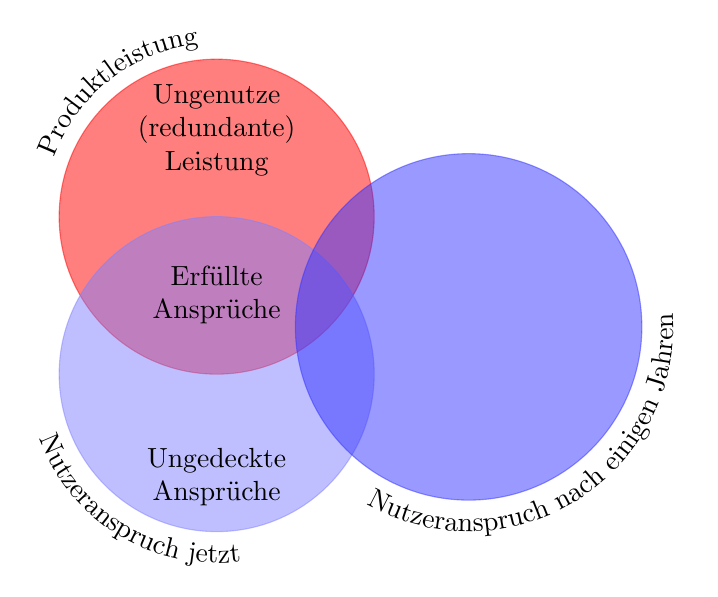
\begin{tikzpicture}[scale=2,
]

\path (0,0)++(0,1.2)++(-1.2,0); %% Bild sonst abgeschnitten

\draw[opacity=.5, red, fill] (0,0) circle(1)++(0,.9)node[below, align=center, text=black, opacity=1]{Ungenutze \\ (redundante) \\ Leistung};
\draw [decorate, decoration={text along path,
text={Produktleistung}}] (0,0) ++ (160:1.1) arc (160:50:1.1);



\draw[opacity=.5, blue!50, fill] (0,-1) circle(1)++(0,-.9)node[above, align=center, text=black, opacity=1]{Ungedeckte \\ Ansprüche};
\draw [decorate, decoration={text along path,
text={Nutzeranspruch jetzt}}] (0,-1) ++ (200:1.2) arc (200:300:1.2);

\path (0,-.5) node[align=center, text=black, opacity=1]{Erfüllte \\ Ansprüche};


\draw[opacity=.5, blue!80, fill] (1.6,-.7)coordinate(x) circle(1.1);
\draw [decorate, decoration={text along path,
text={Nutzeranspruch nach einigen Jahren}}] (x) ++ (240:1.3) arc (240:400:1.3);



\end{tikzpicture}
\end{document}